\section{Markov-Entscheidungsprozess}\label{sec:markov}
Allgemein können Reinforcement-Learning-Probleme mit Hilfe eines Markov"=Entscheidungsprozesses (engl. Markov decision process) \cite[S. 636]{castano} formalisiert werden.

\begin{figure}
    \centering
    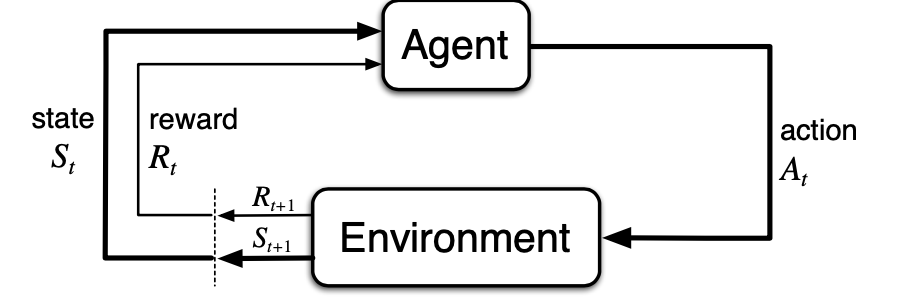
\includegraphics[width=1.0\textwidth]{graphics/markov.png}
    \caption{Ablauf des Markov-Entscheidungsprozess}
    \label{fig:markov_ablauf}
\end{figure}

Der Ablauf wird in \autoref{fig:markov_ablauf} dargestellt und kann laut \cite[S. 636]{castano} als ein \enquote{[...]discrete state-time transition system [...]} beschrieben werden. 
Die zwei Hauptbeteiligten Objekte sind Agent und Umwelt \cite[S. 47ff.]{sutton2018}.
Ein Agent beschreibt eine mit seiner Umwelt interagierende Entität und kann über Software oder Hardware abgebildet werden.
Alle Variablen sind abhängig von diskretisierten Zeitpunkten $t$.
Der Agent erhält zu jedem Zeitpunkt den aktuellen Zustand (engl. state) $s$.
Er kann dann mit der Umwelt z.B. durch Aktoren interagieren, indem er eine Aktion (engl. action) $a \in A_t$ ausführt, wobei die Menge $A_t$ alle Aktionen, die der Agent zum Zeitpunkt $t$ ausführen kann, beschreibt.
Die Wahrscheinlichkeit für den Übergang in den Folgezustand $S_{t+1}$ wird beschrieben durch die Verhaltensstrategie $\pi(a|s_t)$ \cite[S. 58]{sutton2018}.
Für jedes Zustands-Aktions-Paar wird durch eine Belohnungsfunktion eine Belohnung $r_t(s_t, a_t)$ berechnet \cite[S. 638]{castano}.
Ziel ist eine möglichst optimale Abfolge von Aktionen zu ermitteln, um die Summe der Belohnungen zu maximieren.
